\section*{36. Диамагнетики. Гиромагнитное отношение. Ларморовская прецессия.
Оценка магнитной проницаемости.}

\subsection*{Диамагнетики}

\[
1)\chi<0;\qquad2)|\chi|<<1;
\]

\[
\grad(\vec{m}\vec{H})=\grad(-|\chi|H^2)=-|\chi|\grad H^2
\]

\subsection*{Гиромагнитное отношение}

\begin{minipage}[c]{0.4\textwidth} % Левая часть: изображение
    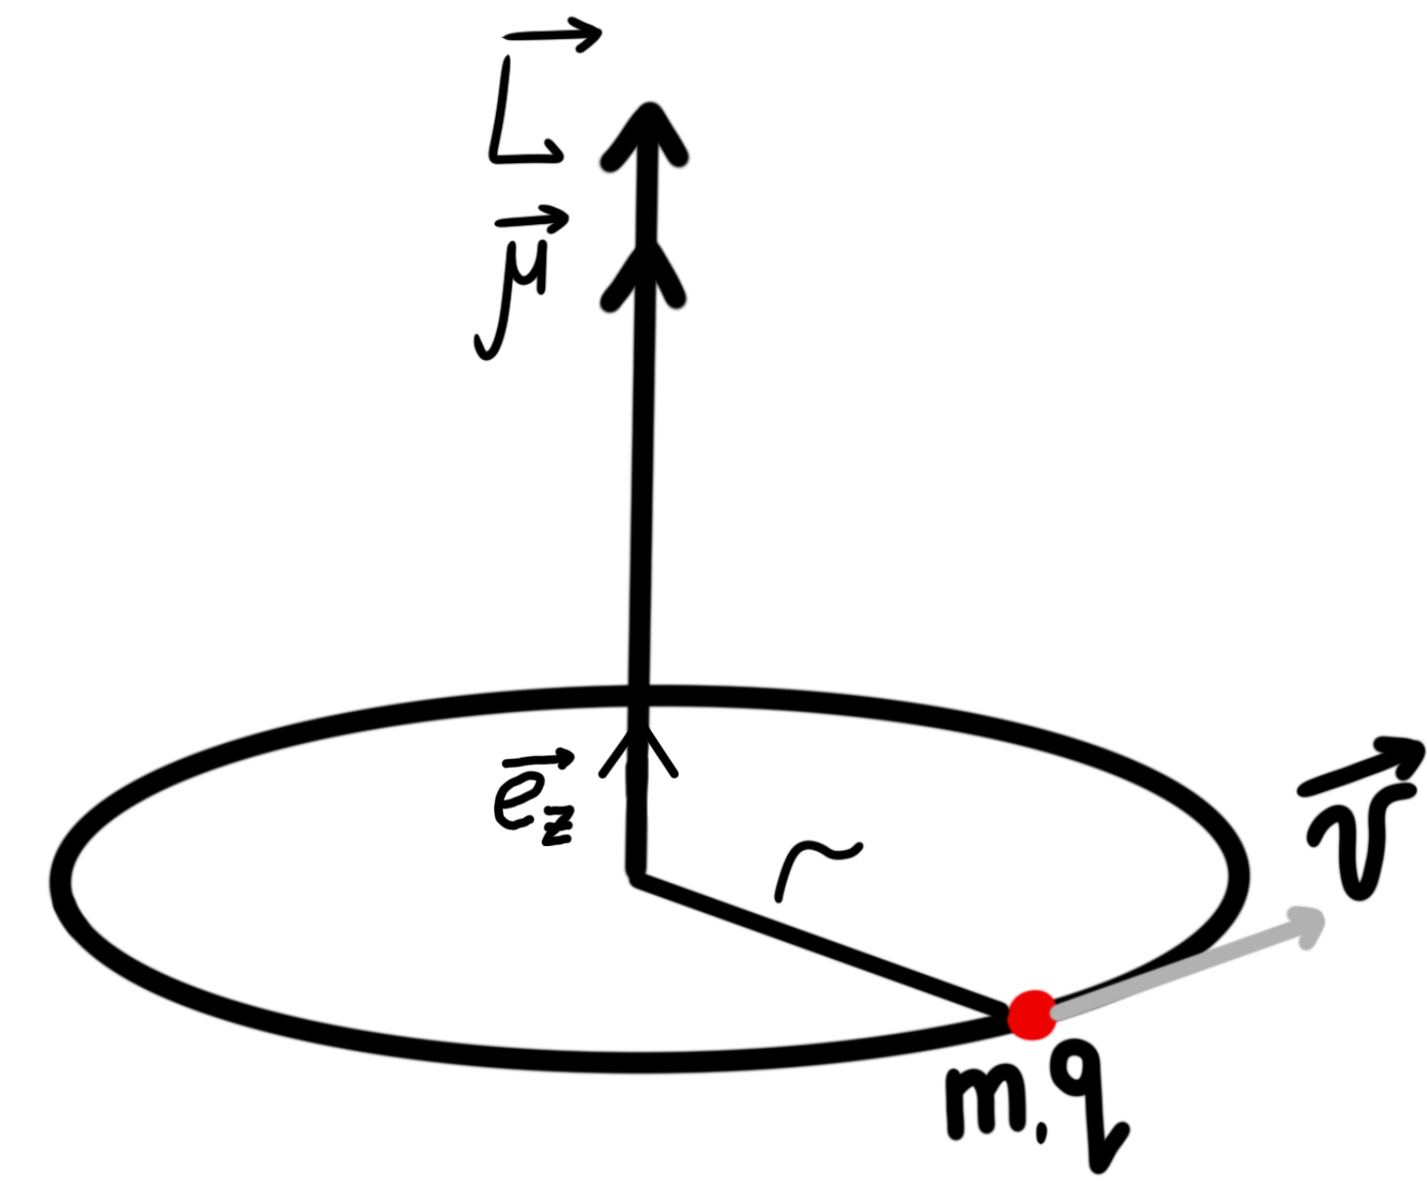
\includegraphics[width=\textwidth]{im/75.png} % Ваше изображение
\end{minipage}%
\hfill
\begin{minipage}[c]{0.6\textwidth} % Правая часть: текст
    \[
    \begin{array}{l|l}
        \vec{\mu}= \frac{I}{c}\vec{S}=\frac{q}{cT}\vec{S}=\frac{q}{cT}\pi r^2 \vec{e_z} & \Rightarrow \\
        \vec{L}=mr\vec{e_z}=\frac{2\pi mr^2}{T}\vec{e_z} 
    \end{array}
    \]
    \[
    \Rightarrow \vec{\mu}=\eta  \vec{L}, \text{ где } \eta=\frac{q}{2mc} 
    \]
    \[
    \eta\text{- гиромагнитное отношение}
    \]
\end{minipage}

\subsection*{Ларморовская прецессия}

\begin{minipage}[c]{0.2\textwidth} % Левая часть: изображение
    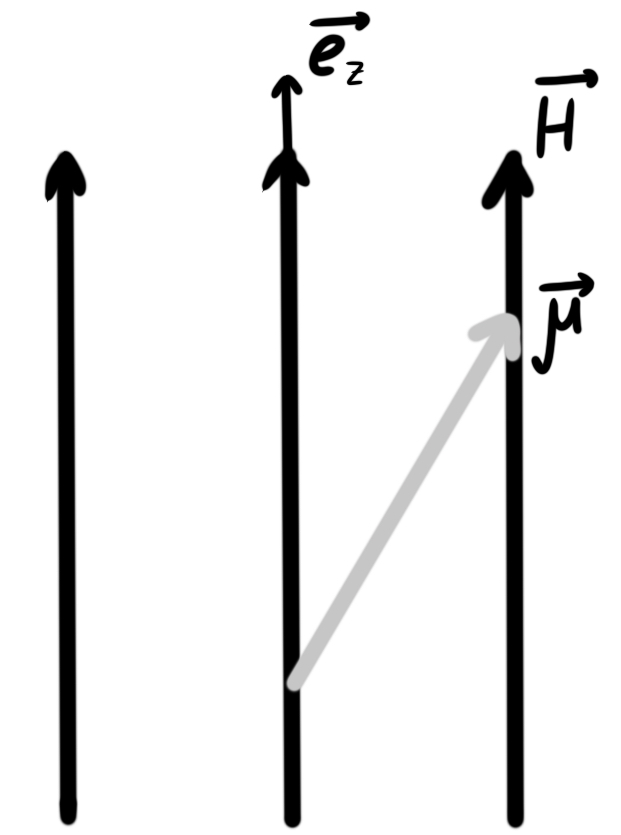
\includegraphics[width=\textwidth]{im/76.png} % Ваше изображение
\end{minipage}%
\hfill
\begin{minipage}[c]{0.6\textwidth} % Правая часть: текст
    \[
    \begin{aligned}
        \frac{d\vec{L}}{dt}=\overset{\text{момент сил}}{\vec{M}}=[\vec{\mu}\times \vec{H}]=[\eta\vec{\nu}\times \vec{H}]=[-\eta\vec{H}\times \vec{L}] \\
        \frac{d\vec{L}}{dt}=[-\eta\vec{H}\times \vec{L}]
    \end{aligned}
    \]
\end{minipage}

\begin{minipage}[c]{0.5\textwidth} % Левая часть: изображение
    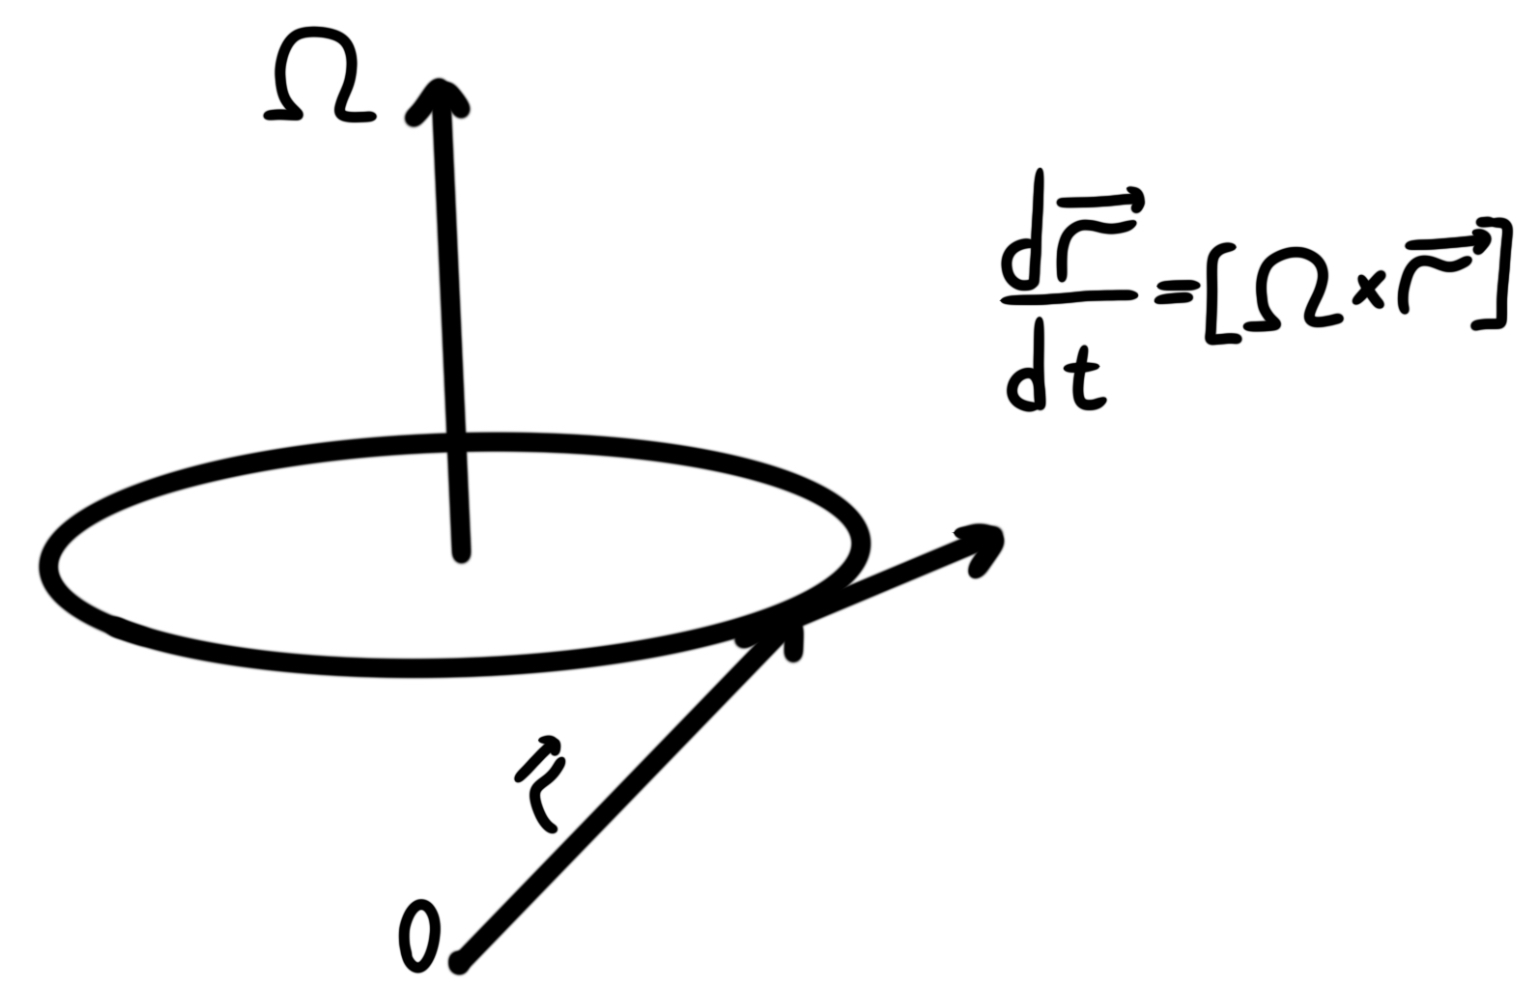
\includegraphics[width=\textwidth]{im/77.png} % Ваше изображение
\end{minipage}%
\hfill
\begin{minipage}[c]{0.6\textwidth} % Правая часть: текст
    \[
     \frac{d\vec{L}}{dt}=[-\eta\vec{H}\times \vec{L}]\Rightarrow\vec{\Omega_{\text{л}}}=-\eta\vec{H}
    \]
\end{minipage}

\subsection*{Оценка магнитной проницаемости}

\[
\Delta \vec{L}=I\vec{\Omega_{\text{л}}},\text{ где } I \text{- момент инерции}
\]

Тогда ветктор намагничености:

\[
\vec{M}=nz\Delta\vec{L}\eta=nzI(-\eta\vec{H})\eta=-nzI\eta^2\vec{H}\Rightarrow \chi=-nzI\eta^2<0
\]

\( n \) -число атомов в единице объема 

\( z \) -число электронов в атоме 